\documentclass[11pt,a4paper]{article}
\usepackage[T1]{fontenc}
\usepackage[utf8]{inputenc}
\usepackage{lmodern}
\usepackage[a4paper,margin=2.4cm]{geometry}
\usepackage{amsmath,amssymb}
\usepackage{booktabs}
\usepackage{graphicx}
\usepackage[font=small,labelfont=bf]{caption}
\usepackage{microtype}
\usepackage[hidelinks]{hyperref}

% Le paquet babel-french n'est pas installé sur les machines de compilation :
% noms des éléments mis en français à la main.
\renewcommand{\figurename}{Figure}
\renewcommand{\tablename}{Tableau}
\renewcommand{\contentsname}{Sommaire}
\renewcommand{\refname}{Références}
\renewcommand{\abstractname}{Résumé}
\newcommand{\og}{\guillemotleft\,\ignorespaces}
\newcommand{\fg}{\unskip\,\guillemotright}

\newcommand{\Lscal}{L_{\mathrm{scal}}}
\newcommand{\Lpred}{L_{\mathrm{pred}}}
\newcommand{\nmse}{\mathrm{nmse}}
\setlength{\parskip}{0.4em}
\setlength{\parindent}{0pt}

\title{Un prédicteur en espace des phases\\pour un \emph{world model} JEPA\\[0.4em]
\large Démarche et résultats, du 28 septembre au 14 octobre 2026}
\author{PSC --- rapport d'étape pour le tuteur}
\date{}

\begin{document}
\maketitle

\begin{abstract}
On part du \emph{world model} LeWM (bibliothèque \texttt{stable-worldmodel}) et du papier
\emph{Temporal Straightening for Latent Planning} (Wang et al., 2026). LeWM-Phase remplace le
prédicteur de LeWM par un prédicteur qui calcule une vitesse latente puis l'intègre
($\hat z_{t+1} = z_t + \hat u_{t+1}$), et ajoute une loss $\Lscal$ qui pousse la réponse du
prédicteur à la vitesse à être un simple multiple de l'identité. Ce document décrit, dans
l'ordre chronologique, les quatre campagnes d'expériences menées (environ 600 entraînements
sur les machines des salles informatiques de l'X), les problèmes rencontrés et ce que chacun
nous a appris. En résumé : LeWM-Phase a d'abord nettement perdu contre LeWM ; on a ensuite
identifié trois causes qui ne tiennent pas à l'idée elle-même (une mémoire plus courte que
LeWM, un protocole de planification qui cachait la vitesse de départ, et une dérive quand on
enchaîne les prédictions). Une fois ces trois points corrigés, LeWM-Phase fait jeu égal avec
LeWM sur MountainCar et le dépasse sur Pendulum en planification par gradient
(89\,\% contre 83\,\%). $\Lscal$ n'a qu'un effet secondaire. Le travail qui a suivi, sur le
\emph{temporal straightening}, n'est pas traité ici.
\end{abstract}

\tableofcontents

%======================================================================
\section{Cadre}
%======================================================================

\subsection{Le modèle de départ : LeWM}

LeWM est un \emph{world model} de type JEPA : il ne prédit pas des images mais des vecteurs
latents.
\begin{itemize}
  \item \textbf{Encodeur} $E$ : un ViT-tiny (12 couches, dimension 192, patchs de
  $14\times14$ pixels, images $224\times224$) suivi d'un MLP. Une image $o_t$ devient un
  vecteur $z_t = E(o_t) \in \mathbb{R}^{192}$ (on garde le token de résumé du ViT).
  \item \textbf{Prédicteur} $f_\theta$ : un transformeur causal de 6 couches. Il reçoit les
  3 derniers vecteurs $z_{t-2}, z_{t-1}, z_t$ et les 3 dernières actions (injectées par
  modulation des couches, dite AdaLN) et prédit $\hat z_{t+1}$.
  \item \textbf{Loss} : $\Lpred = \|\hat z_{t+1} - z_{t+1}\|^2$ (moyenne sur la fenêtre),
  plus un terme anti-effondrement (SIGReg, poids $0{,}09$) qui empêche l'encodeur
  d'envoyer toutes les images sur le même vecteur.
\end{itemize}
Tous nos modèles, LeWM compris, sont entraînés par nous, avec le même budget (même nombre
d'époques, mêmes données, mêmes hyperparamètres ; tableau~\ref{tab:hyper} en annexe). On ne
compare jamais nos modèles au LeWM pré-entraîné 100 époques du papier.

\subsection{Notre modèle : LeWM-Phase}

Le papier étudie un modèle idéalisé $z_{t+1} = A z_t + B a_t$ et montre que la
planification est mieux conditionnée quand $A$ est proche de l'identité. Or $A = I$ donne
$z_{t+1} - z_t = B a_t$ : la vitesse est proportionnelle à l'action, le système s'arrête dès
qu'on cesse d'agir. C'est une physique sans inertie (aristotélicienne). L'idée est de
travailler en espace des phases, comme en mécanique newtonienne. Nous appelons
\textbf{LeWM-Phase} le modèle obtenu (dans nos notes internes, c'était l'\og Idée 9 \fg) :
\begin{align*}
  u_t &= z_t - z_{t-1} && \text{(vitesse latente, calculée, sans paramètre)}\\
  \hat u_{t+1} &= h_\theta(\ldots) && \text{(seule partie apprise)}\\
  \hat z_{t+1} &= z_t + \hat u_{t+1} && \text{(intégration écrite en dur)}
\end{align*}
Deux versions de $h_\theta$ ont été testées :
\begin{itemize}
  \item \textbf{Markov strict} : $h_\theta(z_t, u_t, a_t)$. Le modèle ne voit que 2 images
  ($z_t$ et $z_{t-1}$, à travers $u_t$) et 1 action.
  \item \textbf{Historique} : $h_\theta$ reçoit les 3 derniers couples $(z_i, u_i)$ et les
  3 dernières actions, exactement l'information de LeWM. Seule l'intégration explicite
  $z_t + \hat u_{t+1}$ diffère.
\end{itemize}
Techniquement, $h_\theta$ est le prédicteur de LeWM auquel on donne en entrée la
concaténation $[z_i ; u_i]$ projetée en dimension 192.

\subsection{La loss $\Lscal$}

On note $J_u = \partial h_\theta / \partial u_t$ la réponse du prédicteur à la vitesse.
L'intuition newtonienne est que, sans force, la vitesse se conserve : $J_u$ devrait
ressembler à $\gamma I$. Pour une direction de sonde $w$ ($\|w\|=1$) :
\[
  \hat\gamma(w) = \langle w, J_u w\rangle,\qquad
  \Lscal^{\mathrm{pdf}}(w) = \|J_u w - \hat\gamma(w)\, w\|^2,\qquad
  \Lscal^{\mathrm{inv}}(w) = \frac{\|J_u w - \hat\gamma(w)\, w\|^2}{\|J_u w\|^2}.
\]
$\hat\gamma$ est le meilleur coefficient scalaire le long de $w$. On a $\Lscal(w) = 0$ pour
tout $w$ si et seulement si $J_u = \gamma I$. La version \og pdf \fg{} (celle du document
mathématique de départ) peut baisser simplement en rétrécissant $J_u$ vers 0 ; la version
\og inv \fg{} vaut $\sin^2(w, J_u w)$ et ne dépend que de la forme de $J_u$, pas de sa taille.

Pour calculer $J_u w$ sans construire la matrice $J_u$ (de taille $192\times192$), on appelle
le prédicteur deux fois, avec la vitesse $u_t$ légèrement augmentée puis diminuée dans la
direction $w$, et on fait la différence :
\[
  J_u w \approx \frac{h_\theta(\ldots, u_t + \varepsilon w, \ldots) - h_\theta(\ldots, u_t - \varepsilon w, \ldots)}{2\varepsilon},
  \qquad \varepsilon = 10^{-2}.
\]
On ne perturbe que la dernière vitesse de la fenêtre, celle qui sert à la prédiction utilisée
par le planificateur. Ce calcul est fait en pleine précision : la différence est trop petite
pour la demi-précision utilisée pendant l'entraînement. Enfin, $\Lscal$ ne modifie que le
prédicteur $h_\theta$ : elle ne peut pas faire baisser sa valeur en déformant l'encodeur (par
exemple en écrasant les vitesses). Deux choix de sonde :
\begin{itemize}
  \item \textbf{aléatoire} : $w$ tiré uniformément sur la sphère de $\mathbb{R}^{192}$ ;
  \item \textbf{le long de la vitesse} : $w = u_t/\|u_t\|$, la direction réellement visitée
  (introduite à l'étape~2, voir \S\ref{sec:g9}).
\end{itemize}
Le poids de $\Lscal$ dans la loss totale est noté $\lambda$.

\subsection{Planification et taux de succès}

Le critère final est celui du papier : la planification. On place le simulateur dans un
état de départ, on lui donne une image but, et un planificateur cherche les actions qui
amènent le modèle à prédire l'image but. On exécute ces actions dans le \emph{vrai}
simulateur et on regarde si le but est atteint.
\begin{itemize}
  \item Coût minimisé : $\|\hat z_{t+H} - z_{\text{but}}\|^2$, horizon $H = 5$ blocs, en
  boucle fermée (on replanifie après chaque bloc exécuté).
  \item \textbf{CEM} : 300 séquences d'actions candidates, 30 itérations, on garde les 30
  meilleures. N'utilise pas les dérivées du modèle.
  \item \textbf{Gradient} : Adam (pas $0{,}1$), 50 itérations, 32 initialisations ; les
  actions sont ramenées dans leurs bornes après chaque pas. Il dérive le coût par rapport aux
  actions \emph{à travers} le modèle.
  \item Pour chaque modèle : les \textbf{mêmes 100 problèmes} départ/but, ce qui rend les
  comparaisons appariées.
\end{itemize}
Le succès est jugé sur l'état réel du simulateur (définition précise par environnement plus
bas). Toutes les valeurs sont des moyennes sur les \emph{seeds} (entraînements indépendants
avec des initialisations différentes) $\pm$ l'erreur standard ; $n$ est le nombre de seeds ;
les valeurs de $p$ viennent d'un test de Welch.

\subsection{Vocabulaire}

\begin{center}
\begin{tabular}{@{}lp{11.5cm}@{}}
\toprule
\textbf{Bloc} & Unité de temps du modèle : 5 pas du simulateur (une image et un groupe de 5
actions). \\
\textbf{Mémoire} & Nombre d'images passées que le prédicteur exploite : 2 pour LeWM-Phase
Markov strict, 3 pour LeWM et LeWM-Phase historique. \\
\textbf{Contexte} & Nombre d'images réelles que le planificateur donne au modèle au départ
(1, 2 ou 3). \\
\textbf{Erreur immédiate} & Erreur de prédiction un bloc plus loin, en partant de vraies
images, divisée par la variance de la cible ($\nmse$ ; 0 = parfait). Cette normalisation
rend comparables des modèles dont les espaces latents diffèrent. \\
\textbf{Erreur à $k$ blocs} & Même erreur après $k$ prédictions enchaînées, le modèle
réutilisant ses propres prédictions (comme le planificateur). \\
\textbf{Succès} & Pourcentage des 100 problèmes résolus. \\
\bottomrule
\end{tabular}
\end{center}

\subsection{Moyens de calcul}

Tout tourne sur les machines des salles informatiques de l'X (une carte graphique par
machine, jusqu'à environ 160 machines en parallèle). Règle de la DSI : calcul intensif
seulement la nuit (18\,h--8\,h) et le week-end. En pratique chaque campagne tient en une nuit,
et chaque tâche s'arrête automatiquement à 7\,h\,30.

%======================================================================
\section{Étape 1 (28--30 septembre) : PushT et Reacher}
\label{sec:i9}
%======================================================================

\subsection{Protocole}

\begin{itemize}
  \item \textbf{Configurations} (8) : LeWM ; LeWM-Phase Markov strict sans $\Lscal$ ;
  LeWM-Phase + $\Lscal^{\mathrm{pdf}}$ et + $\Lscal^{\mathrm{inv}}$ avec
  $\lambda \in \{0{,}01\,;\,0{,}1\,;\,1\}$, sonde aléatoire.
  \item \textbf{PushT} (campagne \og i9 \fg{}, nuit du 28 au 29) : un agent pousse un bloc en
  T. Dataset expert du papier (2,3 millions d'images), \textbf{1 époque}, environ 20 seeds
  par configuration, 155 entraînements terminés.
  \item \textbf{Reacher} (DeepMind Control, campagne \og r9 \fg{}, nuit du 29 au 30) : un bras à
  deux segments doit atteindre une cible. \textbf{5 époques} sur 2\,250 des 10\,000 épisodes
  du dataset LeWM, 152 entraînements terminés.
  \item Planification : CEM, contexte d'\textbf{une seule image} (le protocole de
  \texttt{stable-worldmodel}~0.1.1). Le but est l'état atteint 25 pas plus tard dans les
  données ; le planificateur dispose de 50 pas.
\end{itemize}

\subsection{Résultats}

\begin{figure}[htbp]
  \centering
  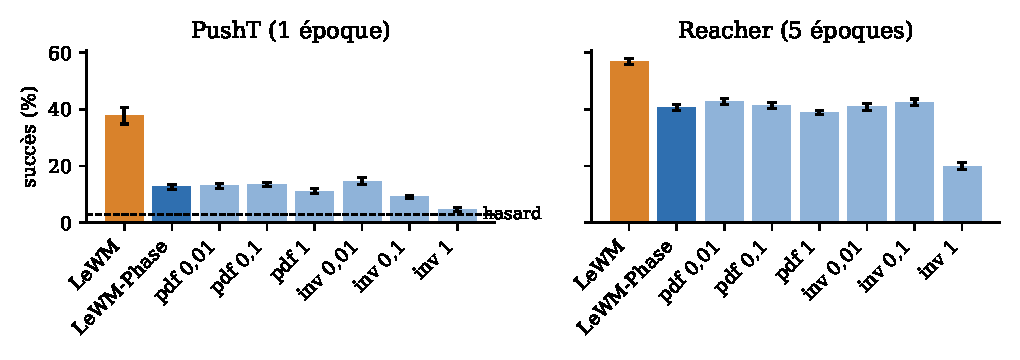
\includegraphics[width=\linewidth]{fig_i9_r9.pdf}
  \caption{Étape 1, succès en planification (CEM, contexte 1 image, 100 problèmes,
  16 à 20 seeds par barre). Orange : LeWM ; bleu foncé : LeWM-Phase Markov strict sans
  $\Lscal$ ; bleu clair : LeWM-Phase + $\Lscal$ (version et $\lambda$ en abscisse).}
  \label{fig:i9r9}
\end{figure}

\begin{table}[htbp]
\centering\small
\begin{tabular}{@{}lrrrrrr@{}}
\toprule
& \multicolumn{3}{c}{PushT (1 époque)} & \multicolumn{3}{c}{Reacher (5 époques)} \\
\cmidrule(lr){2-4}\cmidrule(l){5-7}
Configuration & $n$ & erreur imm. & succès (\%) & $n$ & erreur imm. & succès (\%) \\
\midrule
LeWM                          & 19 & 0,0267 & $37{,}7 \pm 2{,}9$ & 20 & 0,0062 & $56{,}8 \pm 0{,}9$ \\
LeWM-Phase (Markov)               & 19 & 0,0310 & $12{,}7 \pm 0{,}9$ & 20 & 0,0361 & $40{,}5 \pm 1{,}1$ \\
+ $\Lscal^{\mathrm{pdf}}$, $\lambda=0{,}01$ & 19 & 0,0311 & $13{,}0 \pm 0{,}8$ & 19 & 0,0362 & $42{,}8 \pm 1{,}1$ \\
+ $\Lscal^{\mathrm{pdf}}$, $\lambda=0{,}1$  & 20 & 0,0318 & $13{,}4 \pm 0{,}7$ & 19 & 0,0366 & $41{,}2 \pm 1{,}1$ \\
+ $\Lscal^{\mathrm{pdf}}$, $\lambda=1$      & 19 & 0,0374 & $11{,}2 \pm 0{,}8$ & 19 & 0,0405 & $38{,}8 \pm 0{,}7$ \\
+ $\Lscal^{\mathrm{inv}}$, $\lambda=0{,}01$ & 18 & 0,0309 & $14{,}7 \pm 1{,}2$ & 20 & 0,0361 & $40{,}8 \pm 1{,}2$ \\
+ $\Lscal^{\mathrm{inv}}$, $\lambda=0{,}1$  & 18 & 0,0526 & $9{,}2 \pm 0{,}5$  & 16 & 0,0383 & $42{,}5 \pm 1{,}1$ \\
+ $\Lscal^{\mathrm{inv}}$, $\lambda=1$      & 19 & 0,0849 & $4{,}6 \pm 0{,}7$  & 19 & 0,1300 & $19{,}9 \pm 1{,}2$ \\
\midrule
Politique aléatoire & & & 3,0 & & & non mesurée \\
\bottomrule
\end{tabular}
\caption{Étape 1. Erreur immédiate en validation et succès en planification.}
\label{tab:i9r9}
\end{table}

\begin{itemize}
  \item \textbf{LeWM-Phase perd nettement} : $-25$ points sur PushT ($37{,}7 \to 12{,}7\,\%$,
  $p = 5\cdot10^{-8}$) et $-16$ points sur Reacher ($56{,}8 \to 40{,}5\,\%$,
  $p = 4\cdot10^{-13}$). Sur Reacher, son erreur immédiate est 6 fois celle de LeWM.
  \item \textbf{$\Lscal$ n'apporte aucun gain significatif.} Pour $\lambda \le 0{,}1$, les
  écarts avec LeWM-Phase seul ne sont pas significatifs ($p \ge 0{,}14$), sauf la version inv à
  $\lambda = 0{,}1$ sur PushT, significativement moins bonne ($9{,}2$ contre $12{,}7\,\%$,
  $p = 0{,}002$). À $\lambda = 1$, $\Lscal$ dégrade tout.
  \item \textbf{Ce que $\Lscal$ fait à $J_u$} (Reacher). La version pdf à $\lambda=1$ divise
  la taille de $J_u w$ par 4 ($0{,}23 \to 0{,}053$) sans le rendre plus scalaire : c'est la
  solution triviale prévue ($J_u \to 0$). La version inv à $\lambda = 0{,}1$ rend bien $J_u$
  presque scalaire ($\sin^2$ moyen $0{,}995 \to 0{,}21$), mais avec $\hat\gamma = -0{,}29$ :
  une vitesse qui s'inverse à chaque bloc, ce qui n'a pas de sens physique. Même constat sur
  PushT ($\hat\gamma = -0{,}06$).
\end{itemize}

\subsection{Problèmes rencontrés}

\begin{itemize}
  \item \textbf{Biais du protocole sur PushT.} Le planificateur ne donne qu'une image au
  départ, donc $u_0$ est inconnu ; on le met à 0. Les modèles LeWM-Phase de PushT n'avaient jamais
  vu $u = 0$ à l'entraînement. Pour Reacher, on a corrigé ce point en entraînant aussi sur la
  position où $u_0 = 0$. L'écart avec LeWM est resté de 16 points.
  \item \textbf{Une conclusion fausse.} Avec des sondes aléatoires, $\hat\gamma \approx 0$
  et $\|J_u w\|$ petit. On en avait conclu que le prédicteur \og ignore la vitesse \fg{}. C'était
  trop fort : en dimension 192, une sonde aléatoire tombe presque toujours hors des quelques
  directions où $J_u$ agit vraiment, et $\hat\gamma$ mesure alors à peu près
  $\mathrm{tr}(J_u)/192$. L'étape suivante mesure $J_u$ le long de $u_t$.
\end{itemize}

\textbf{Questions laissées ouvertes} : (1) l'écart vient-il de l'intégration explicite ou
simplement de la mémoire plus courte (2 images au lieu de 3) ? (2) le prédicteur
utilise-t-il la vitesse ? (3) sur PushT, presque statique, l'inertie n'a de toute façon
aucun rôle : il faut un environnement où elle compte.

%======================================================================
\section{Étape 2 (7--9 octobre) : environnements à inertie, mémoire 3}
\label{sec:g9}
%======================================================================

\subsection{Nouveaux environnements}

On a supprimé PushT et Reacher (place disque) et créé deux tâches à partir de Gymnasium, où
la vitesse est la moitié de l'état :
\begin{itemize}
  \item \textbf{Pendulum} : un pendule actionné par un couple $\in [-2, 2]$. État
  $(\theta, \dot\theta)$. Il tourne vite : il bouge nettement d'une image à l'autre.
  \item \textbf{MountainCar} (version continue) : une voiture dans une vallée, force
  $\in [-1, 1]$, trop faible pour monter directement : il faut prendre de l'élan. État
  $(x, \dot x)$. Mouvement lent et régulier.
  \item \textbf{Données} : aucun dataset n'existait, on les a collectés : 3\,000 épisodes de
  200 pas par environnement, images $224\times224$ sans indicateur de l'action à l'écran,
  actions tirées d'un bruit corrélé dans le temps (Ornstein--Uhlenbeck, $\rho = 0{,}9$) pour
  produire de vrais mouvements avec élan, états initiaux tirés largement.
  \item \textbf{Critère de succès} : être à la position du but \textbf{exactement au pas 25}
  (5 blocs) : $|\theta - \theta_{\text{but}}| < 0{,}15$\,rad pour Pendulum,
  $|x - x_{\text{but}}| < 0{,}02$ pour MountainCar (piste de longueur 1,8). On n'utilise que
  des buts non triviaux (au moins $0{,}5$\,rad, ou $0{,}1$, du départ). Le critère est
  réalisable : rejouer les actions des données réussit à 100\,\%, et un \og oracle \fg{} qui
  planifie avec le vrai simulateur aussi. Une politique aléatoire fait 10 à 16\,\%.
\end{itemize}
\textbf{Échec en route} : notre premier critère (\og passer par le but à un moment
quelconque \fg{}) donnait 83\,\% de succès à une politique aléatoire. Il a été abandonné.

\subsection{Protocole (campagne \og g9 \fg{}, nuit du 7 au 8)}

6 configurations, 5 époques, 12 à 13 seeds chacune, 153 entraînements :
LeWM ; LeWM-Phase Markov strict (mémoire 2) ; LeWM-Phase historique (mémoire 3) ; LeWM-Phase historique +
$\Lscal^{\mathrm{inv}}$ avec sonde le long de $u_t$ ($\lambda = 0{,}01$ et $0{,}1$) ou sonde
aléatoire ($\lambda = 0{,}1$). Nouvelle mesure, sans effet sur l'entraînement :
\begin{itemize}
  \item \textbf{$J_u$ le long de $u_t$} : gain $\|J_u w\|$ et alignement $\cos(w, J_u w)$ pour
  $w = u_t/\|u_t\|$.
\end{itemize}
Planification : CEM, contexte d'une image, comme à l'étape 1.

\subsection{Résultats}

\begin{table}[htbp]
\centering\small
\begin{tabular}{@{}lcccccc@{}}
\toprule
& \multicolumn{3}{c}{Pendulum} & \multicolumn{3}{c}{MountainCar} \\
\cmidrule(lr){2-4}\cmidrule(l){5-7}
Configuration & erreur imm. & succès (\%) & $n$ & erreur imm. & succès (\%) & $n$ \\
\midrule
LeWM                                  & 0,0171 & $16{,}8 \pm 0{,}9$ & 13 & 0,0117 & $12{,}0 \pm 0{,}7$ & 13 \\
LeWM-Phase, mémoire 2                     & 0,1653 & $11{,}5 \pm 0{,}7$ & 13 & 0,0498 & $13{,}5 \pm 0{,}9$ & 13 \\
LeWM-Phase, mémoire 3                     & 0,0163 & $11{,}6 \pm 0{,}6$ & 13 & 0,0100 & $12{,}4 \pm 0{,}8$ & 13 \\
\quad + $\Lscal$, sonde $u$, $\lambda=0{,}01$ & 0,0172 & $15{,}0 \pm 1{,}4$ & 12 & 0,0099 & $13{,}6 \pm 0{,}8$ & 13 \\
\quad + $\Lscal$, sonde $u$, $\lambda=0{,}1$  & 0,0153 & $13{,}4 \pm 1{,}1$ & 13 & 0,0112 & $13{,}4 \pm 0{,}7$ & 12 \\
\quad + $\Lscal$, sonde aléatoire, $\lambda=0{,}1$ & 0,0192 & $9{,}7 \pm 0{,}8$ & 13 & 0,0126 & $13{,}0 \pm 0{,}8$ & 12 \\
\midrule
Politique aléatoire & & 10,0 & & & 13,0 & \\
\bottomrule
\end{tabular}
\caption{Étape 2 (5 époques). Succès : CEM, contexte 1 image.}
\label{tab:g9}
\end{table}

\begin{itemize}
  \item \textbf{La mémoire expliquait l'essentiel de l'écart en prédiction.} Avec 2 images,
  LeWM-Phase prédit 4 à 10 fois moins bien que LeWM. Avec 3 images, il fait aussi bien sur
  Pendulum (0,0163 contre 0,0171) et mieux sur MountainCar (0,0100 contre 0,0117,
  $p = 7\cdot 10^{-10}$). Les mauvais résultats de l'étape 1 venaient donc en grande partie de
  ce qu'on comparait un modèle à 2 images à un modèle à 3 images. Toutes les expériences
  suivantes utilisent la version historique.
  \item \textbf{Le prédicteur utilise fortement la vitesse.} Le long de $u_t$, le gain de $J_u$ vaut $1{,}34$ contre $0{,}48$ dans une
  direction aléatoire (Pendulum). Mais la réponse est presque perpendiculaire à $u_t$
  ($\cos \approx 0{,}01$) : $J_u$ fait tourner la vitesse au lieu de la conserver, ce qui est
  cohérent avec un pendule.
  \item \textbf{Quand $\Lscal$ (sonde $u$, $\lambda = 0{,}1$) impose un $J_u$ scalaire, elle y
  arrive} ($\sin^2$ le long de $u_t$ : $0{,}91 \to 0{,}014$), \textbf{mais toujours avec un
  $\gamma$ négatif} : $\hat\gamma = -0{,}27$ (Pendulum) et $-0{,}23$ (MountainCar), soit
  $J_u u_t \approx -0{,}27\, u_t$.
  \item \textbf{Surprise : en planification, tous les modèles sont au niveau du hasard}, LeWM
  compris (16,8\,\% contre 10\,\% sur Pendulum ; 12,0\,\% contre 13\,\% sur MountainCar),
  alors qu'ils prédisent bien. Le problème est donc dans le protocole, pas dans les modèles.
  Hypothèse : avec une seule image au départ, le planificateur ne connaît pas la vitesse
  initiale, qui est la moitié de l'état.
\end{itemize}

%======================================================================
\section{Étape 3 (10 octobre) : réévaluation et mesure de la dérive}
\label{sec:ev2}
%======================================================================

\subsection{Contexte du planificateur et choix de l'optimiseur}

On a réévalué les modèles de l'étape 2, sans les réentraîner, en faisant varier :
\begin{itemize}
  \item le \textbf{contexte} : 1, 2 ou 3 images réelles au départ, avec les actions exécutées
  entre elles (le passé est pris dans les données : c'est la trajectoire qui mène à l'état de
  départ) ;
  \item l'\textbf{optimiseur} : CEM ou gradient.
\end{itemize}
Pourquoi comparer les deux optimiseurs : jusqu'ici on n'utilisait que le CEM (le réglage par
défaut de \texttt{stable-worldmodel}). Or toute la démonstration du papier \emph{Temporal
Straightening} porte sur la planification \emph{par gradient} : son théorème dit qu'un espace
latent plus \og droit \fg{} rend le problème d'optimisation des actions mieux conditionné, donc
plus facile pour une descente de gradient. Le CEM, lui, n'utilise jamais les dérivées du modèle
et ne profite pas directement de cet argument. Pour pouvoir relier nos résultats à ceux du
papier, il fallait donc évaluer aussi avec le gradient.

Un oracle qui planifie avec le vrai simulateur résout 100\,\% des problèmes ; la politique
aléatoire en résout 16\,\%.

\begin{table}[htbp]
\centering\small
\begin{tabular}{@{}lcccccc@{}}
\toprule
& \multicolumn{3}{c}{Gradient} & \multicolumn{3}{c}{CEM} \\
\cmidrule(lr){2-4}\cmidrule(l){5-7}
Configuration & 1 image & 2 images & 3 images & 1 image & 2 images & 3 images \\
\midrule
\multicolumn{7}{@{}l}{\emph{Pendulum}} \\
LeWM                    & 16,0 & 67,9 & 66,7 & 16,6 & \textbf{80,6} & \textbf{81,1} \\
LeWM-Phase, mémoire 2       & 14,2 & 34,4 & 34,6 & 13,7 & 29,5 & 29,3 \\
LeWM-Phase, mémoire 3       & 12,9 & 68,8 & 68,8 & 12,6 & 75,4 & 74,5 \\
\quad + $\Lscal$, sonde $u$, $\lambda = 0{,}01$ & 15,3 & \textbf{72,5} & 71,2 & 16,8 & 78,6 & 78,5 \\
\quad + $\Lscal$, sonde $u$, $\lambda = 0{,}1$  & 15,3 & 70,5 & \textbf{71,8} & 12,6 & 77,1 & 79,0 \\
\quad + $\Lscal$, sonde aléatoire, $\lambda = 0{,}1$ & 13,3 & 70,6 & 71,5 & 12,8 & 77,1 & 77,9 \\
\midrule
\multicolumn{7}{@{}l}{\emph{MountainCar}} \\
LeWM                    & 12,6 & \textbf{70,6} & \textbf{67,8} & 10,8 & \textbf{73,8} & \textbf{74,6} \\
LeWM-Phase, mémoire 2       & 9,3  & 24,8 & 24,7 & 11,9 & 25,5 & 25,4 \\
LeWM-Phase, mémoire 3       & 9,9  & 42,7 & 43,5 & 13,0 & 45,9 & 45,7 \\
\quad + $\Lscal$, sonde $u$, $\lambda = 0{,}01$ & 10,8 & 43,4 & 42,0 & 11,8 & 45,7 & 45,6 \\
\quad + $\Lscal$, sonde $u$, $\lambda = 0{,}1$  & 11,4 & 47,8 & 44,8 & 13,3 & 49,6 & 47,2 \\
\quad + $\Lscal$, sonde aléatoire, $\lambda = 0{,}1$ & 10,6 & 46,2 & 45,4 & 11,3 & 46,8 & 46,8 \\
\bottomrule
\end{tabular}
\caption{Étape 3. Succès (\%) des modèles de l'étape 2 selon le contexte et l'optimiseur
(11 à 13 seeds par case ; erreurs standards entre 0,2 et 2,5 points). Oracle : 100\,\% ;
hasard : 16\,\%.}
\label{tab:ev2}
\end{table}

\begin{itemize}
  \item \textbf{Le contexte est décisif.} Avec 1 image, tout le monde reste au niveau du
  hasard. Dès 2 images, la vitesse de départ est connue et LeWM passe à 68--81\,\%. La
  3\textsuperscript{e} image n'apporte rien. À partir d'ici, tous les résultats sont donnés avec
  un contexte de 2 images.
  \item \textbf{Sur Pendulum, LeWM-Phase (mémoire 3) fait jeu égal avec LeWM} au gradient
  (68,8 contre 67,9\,\%) et $\Lscal$ ajoute 2 à 5 points
  ($p = 10^{-3}$ pour $\lambda = 0{,}01$ contre LeWM). Au CEM, LeWM reste devant de 2 à 5 points.
  \item \textbf{Sur MountainCar, LeWM-Phase reste loin derrière} : 43 à 48\,\% contre 71--74\,\%
  ($p < 10^{-6}$), alors que son erreur immédiate est la plus basse. D'où la mesure suivante.
\end{itemize}

\subsection{Erreur à plusieurs blocs : la dérive}

On a mesuré l'erreur à $k$ blocs ($k = 1, \ldots, 5$) sur 4\,096 fenêtres tirées des données :
à partir de 3 vraies images, le modèle enchaîne $k$ prédictions en réutilisant les siennes,
comme le fait le planificateur. Courbes pleines de la figure~\ref{fig:derive}.

\begin{table}[htbp]
\centering\small
\begin{tabular}{@{}lccccc|ccccc@{}}
\toprule
& \multicolumn{5}{c|}{Pendulum} & \multicolumn{5}{c}{MountainCar} \\
Configuration & $k{=}1$ & 2 & 3 & 4 & 5 & $k{=}1$ & 2 & 3 & 4 & 5 \\
\midrule
LeWM                         & 0,017 & 0,050 & 0,162 & 0,327 & 0,446 & 0,012 & 0,021 & 0,045 & 0,090 & \textbf{0,151} \\
LeWM-Phase, mémoire 2            & 0,165 & 0,460 & 0,769 & 0,936 & 1,107 & 0,051 & 0,163 & 0,403 & 0,722 & 0,998 \\
LeWM-Phase, mémoire 3            & 0,016 & 0,068 & 0,195 & 0,337 & 0,493 & 0,010 & 0,031 & 0,103 & 0,245 & 0,435 \\
\quad + $\Lscal$, $u$, $0{,}1$  & 0,015 & 0,040 & 0,108 & 0,221 & \textbf{0,334} & 0,011 & 0,028 & 0,084 & 0,184 & 0,312 \\
\quad + $\Lscal$, aléat., $0{,}1$ & 0,019 & 0,046 & 0,120 & 0,244 & 0,367 & 0,012 & 0,028 & 0,081 & 0,168 & 0,298 \\
\bottomrule
\end{tabular}
\caption{Étape 3. Erreur à $k$ blocs des modèles de l'étape 2 (7 à 11 seeds par ligne).}
\label{tab:derive}
\end{table}

\begin{itemize}
  \item \textbf{Sur MountainCar, LeWM-Phase dérive.} Il est le meilleur à 1 bloc mais son erreur
  croît beaucoup plus vite : à 5 blocs (l'horizon du planificateur), elle vaut 0,435 contre
  0,151 pour LeWM, près de 3 fois plus. Explication probable : dans
  $\hat z_{t+1} = z_t + \hat u_{t+1}$, une erreur sur la vitesse s'ajoute à la position et n'est
  jamais corrigée. C'est cohérent avec ses $-28$ points de succès.
  \item \textbf{$\Lscal$ réduit cette dérive d'environ 30\,\%} (0,435 $\to$ 0,312 sur MountainCar ;
  0,493 $\to$ 0,334 sur Pendulum), avec la sonde $u$ comme avec la sonde aléatoire. C'est son
  seul effet net jusqu'ici.
  \item Sur Pendulum, LeWM dérive presque autant que LeWM-Phase : l'écart y est masqué.
  \item Pour donner l'échelle : prédire \og l'image ne change pas \fg{} donne une erreur à
  5 blocs d'environ 1,9.
\end{itemize}

%======================================================================
\section{Étape 4 (13--14 octobre) : loss sur plusieurs blocs}
\label{sec:m9}
%======================================================================

\subsection{Idée et protocole (campagne \og m9 \fg{})}

Puisque le planificateur enchaîne 5 prédictions, on entraîne le modèle à le faire. Pour une
fenêtre de 8 images, à partir des 3 premières vraies images, le modèle enchaîne $K = 5$
prédictions avec les vraies actions, en réutilisant les siennes, et on pénalise l'erreur
moyenne :
\[
  L_{\mathrm{multi}} = \frac{1}{K}\sum_{k=1}^{K} \bigl\|\hat z_{t+k} - z_{t+k}\bigr\|^2,
  \qquad L = \Lpred + L_{\mathrm{multi}} + 0{,}09\, L_{\mathrm{SIGReg}} \;(+\,\lambda\,\Lscal).
\]
Le gradient traverse toute la chaîne de prédictions. Trois configurations sur les deux
environnements : LeWM, LeWM-Phase (mémoire 3), LeWM-Phase + $\Lscal^{\mathrm{inv}}$ (sonde $u$,
$\lambda = 0{,}1$) ; 5 époques. Évaluation : gradient et CEM, contexte 2 et 3 images, plus
l'erreur à $k$ blocs.

\subsection{Problèmes rencontrés}

Cette campagne a été la plus difficile à faire tourner.
\begin{itemize}
  \item \textbf{Mémoire de la carte graphique} : les fenêtres de 8 images au lieu de 4
  demandaient 19,2\,Go et dépassaient la mémoire de certaines cartes. Corrigé en recalculant les
  activations de l'encodeur pendant la rétropropagation (\emph{gradient checkpointing}) :
  6,7\,Go, gradients identiques, environ 30\,\% de calcul en plus.
  \item \textbf{Mémoire vive} : le chargement des données en parallèle montait à 37\,Go de RAM
  et faisait tuer le processus. Corrigé en réduisant le préchargement (3\,Go).
  \item \textbf{Une erreur de notre part} : un script de suivi défectueux a supprimé les dossiers
  de résultats de 131 entraînements en cours. Il a fallu tout arrêter et tout relancer.
  \item \textbf{Conséquence} : la campagne est repartie tard dans la nuit. Un entraînement dure
  environ 6\,h ; beaucoup n'ont pas été au bout, ou ont été coupés par l'arrêt automatique de
  7\,h\,30 pendant leur évaluation. Sur 133 entraînements lancés, seuls 5 à 8 par configuration ont été entraînés et évalués en
  entier ; l'erreur à $k$ blocs complète n'est disponible que pour 1 à 4 seeds.
\end{itemize}

\subsection{Résultats}

\begin{figure}[htbp]
  \centering
  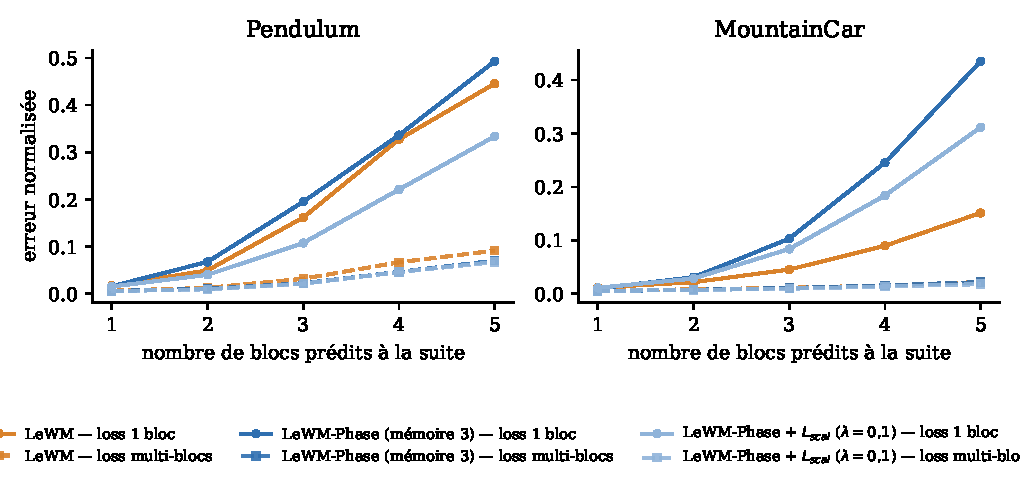
\includegraphics[width=\linewidth]{fig_derive.pdf}
  \caption{Erreur à $k$ blocs. Traits pleins : modèles de l'étape 2 (loss à 1 bloc,
  7 à 11 seeds). Tirets : loss multi-blocs (étape 4, 1 à 4 seeds). Même couleur = même
  configuration.}
  \label{fig:derive}
\end{figure}

\begin{table}[htbp]
\centering\small
\begin{tabular}{@{}llcccc@{}}
\toprule
& & \multicolumn{2}{c}{Pendulum} & \multicolumn{2}{c}{MountainCar} \\
\cmidrule(lr){3-4}\cmidrule(l){5-6}
& Configuration & loss 1 bloc & loss multi-blocs & loss 1 bloc & loss multi-blocs \\
\midrule
Erreur immédiate & LeWM            & 0,0171 & 0,0066 & 0,0117 & 0,0063 \\
                 & LeWM-Phase          & 0,0163 & 0,0062 & 0,0100 & \textbf{0,0048} \\
                 & LeWM-Phase + $\Lscal$ & 0,0153 & \textbf{0,0059} & 0,0112 & 0,0057 \\
\midrule
Erreur à 5 blocs & LeWM            & 0,446 & 0,092 & 0,151 & 0,022 \\
                 & LeWM-Phase          & 0,493 & 0,070 & 0,435 & 0,022 \\
                 & LeWM-Phase + $\Lscal$ & 0,334 & \textbf{0,067} & 0,312 & \textbf{0,018} \\
\midrule
Succès, gradient   & LeWM            & $67{,}9$ & $82{,}8 \pm 1{,}2$ (6) & $70{,}6$ & $\mathbf{84{,}7 \pm 1{,}4}$ (7) \\
(2 images, \%)     & LeWM-Phase          & $68{,}8$ & $\mathbf{89{,}4 \pm 0{,}7}$ (8) & $42{,}7$ & $83{,}3 \pm 1{,}0$ (7) \\
                   & LeWM-Phase + $\Lscal$ & $70{,}5$ & $87{,}5 \pm 1{,}3$ (6) & $47{,}8$ & $80{,}2 \pm 1{,}8$ (5) \\
\midrule
Succès, CEM        & LeWM            & $80{,}6$ & $76{,}8 \pm 0{,}9$ (6) & $73{,}8$ & $\mathbf{76{,}2 \pm 1{,}1}$ (6) \\
(2 images, \%)     & LeWM-Phase          & $75{,}4$ & $78{,}5 \pm 1{,}3$ (6) & $45{,}9$ & $73{,}5 \pm 2{,}0$ (6) \\
                   & LeWM-Phase + $\Lscal$ & $77{,}1$ & $\mathbf{78{,}8 \pm 1{,}4}$ (5) & $49{,}6$ & $73{,}7 \pm 2{,}8$ (3) \\
\bottomrule
\end{tabular}
\caption{Étape 4 comparée aux mêmes configurations entraînées avec la loss à 1 bloc
(étape~2, 12--13 seeds ; succès de l'étape~3). 5 époques dans les deux cas. Entre parenthèses :
nombre de seeds. Avec 3 images de contexte, le gradient donne 83,7 / 90,4 / 89,2\,\% (Pendulum)
et 87,0 / 88,5 / 87,8\,\% (MountainCar).}
\label{tab:m9}
\end{table}

\begin{itemize}
  \item \textbf{La loss multi-blocs fait disparaître la dérive} : l'erreur à 5 blocs est divisée
  par 5 à 20, et celle de LeWM-Phase sur MountainCar tombe de 0,435 à 0,022, au niveau de LeWM.
  L'erreur immédiate est aussi divisée par 2 à 2,6 pour tous les modèles.
  \item \textbf{En planification par gradient, tout le monde progresse fortement}, de +14 points
  (LeWM, MountainCar) à +41 points (LeWM-Phase, MountainCar). LeWM-Phase rattrape LeWM sur MountainCar
  (83,3 contre 84,7\,\%) et le dépasse sur Pendulum (89,4 contre 82,8\,\%, soit +6,6 points
  avec des erreurs standards d'environ 1 point).
  \item \textbf{Avec le CEM, les gains sont bien plus faibles.} LeWM ne progresse pas
  (Pendulum $80{,}6 \to 76{,}8\,\%$, MountainCar $73{,}8 \to 76{,}2\,\%$) ; seul LeWM-Phase sur
  MountainCar, débarrassée de sa dérive, remonte ($45{,}9 \to 73{,}5\,\%$). Tous les modèles
  plafonnent entre 73 et 79\,\%, en dessous du gradient. Un modèle fidèle sur plusieurs blocs
  profite surtout à l'optimiseur qui utilise ses dérivées, ce qui est cohérent avec l'argument
  du papier sur le conditionnement de la planification par gradient.
  \item \textbf{$\Lscal$ n'apporte rien de mesurable en plus} de la loss multi-blocs : ses
  résultats sont dans les barres d'erreur de LeWM-Phase seul.
\end{itemize}

%======================================================================
\section{Bilan}
%======================================================================

\begin{table}[htbp]
\centering\small
\begin{tabular}{@{}lp{12.3cm}@{}}
\toprule
Variable & Effet mesuré \\
\midrule
Contexte & Décisif. 1 image : tous les modèles au niveau du hasard (10--16\,\%). 2 images :
LeWM à 68--81\,\%. La 3\textsuperscript{e} image n'apporte rien. \\
Mémoire & LeWM-Phase a besoin de 3 images comme LeWM. Avec 2, son erreur immédiate est 4 à
10 fois plus grande. \\
Intégration explicite & À mémoire égale, LeWM-Phase prédit aussi bien ou mieux que LeWM à
1 bloc, mais dérive quand on enchaîne les prédictions (MountainCar : erreur à 5 blocs $\times 3$). \\
$\Lscal$ & Réduit la dérive d'environ 30\,\% ; quelques points de succès au mieux ; inutile
une fois la loss multi-blocs ajoutée. Quand elle rend $J_u$ scalaire, $\gamma$ est toujours
négatif, ce qui n'a pas de sens physique. \\
Loss multi-blocs & Le levier le plus fort : erreur à 5 blocs divisée par 5 à 20, succès au
gradient +14 à +41 points. \\
Optimiseur & Le gradient profite des modèles fidèles sur plusieurs blocs (jusqu'à 89\,\%) ;
le CEM plafonne à 73--79\,\%. \\
\bottomrule
\end{tabular}
\caption{Ce que chaque variable a changé, sur l'ensemble des quatre étapes.}
\end{table}

\textbf{Ce que l'on peut affirmer.} LeWM-Phase n'est pas mauvais en soi. Ses mauvais résultats
initiaux venaient de trois causes extérieures à l'idée : une mémoire plus courte que LeWM, un
protocole de planification qui cachait la vitesse de départ, et une dérive d'intégration que la
loss multi-blocs corrige. Avec ces corrections, il égale LeWM sur MountainCar et le dépasse
sur Pendulum en planification par gradient. $\Lscal$, l'objet de départ, n'a qu'un rôle
secondaire.

\textbf{Limites.}
\begin{itemize}
  \item Les résultats de l'étape 4 reposent sur 5 à 8 seeds par configuration (contre 12 à 20
  aux étapes précédentes). L'avance de LeWM-Phase sur Pendulum est à confirmer.
  \item Entraînements courts : 5 époques (1 pour PushT), contre 100 dans le papier.
  \item Données collectées au hasard, et non par un expert.
  \item Horizon de planification court (5 blocs, soit 25 pas).
  \item Les erreurs immédiates sont normalisées par la variance de la cible, mais restent
  calculées dans des espaces latents différents : seul le succès en planification compare
  vraiment les modèles.
\end{itemize}

\textbf{Suite.} L'étape suivante, non traitée ici, a consisté à ajouter la loss de courbure
$L_{\mathrm{curv}}$ du papier \emph{Temporal Straightening}, puis un latent par patchs.

%======================================================================
\appendix
\section{Hyperparamètres communs}
%======================================================================

\begin{table}[htbp]
\centering\small
\begin{tabular}{@{}lp{12.2cm}@{}}
\toprule
Encodeur & ViT-tiny (12 couches, 3 têtes, dimension 192), patchs $14\times14$, images
$224\times224$, entraîné depuis zéro \\
Projecteurs & MLP $192 \to 2048 \to 192$ avec BatchNorm \\
Prédicteur & transformeur causal, 6 couches, 16 têtes de dimension 64, MLP 2048,
dropout 0,1, actions en AdaLN \\
Mémoire / fenêtre & 3 images ; fenêtre de 4 images (8 avec la loss multi-blocs) \\
Bloc & 5 pas du simulateur (\emph{frameskip} 5) \\
Optimisation & AdamW, taux d'apprentissage $5\cdot10^{-5}$, \emph{weight decay} $10^{-3}$,
batch 128, préchauffage 1\,\% puis décroissance en cosinus, bf16, écrêtage du gradient à 1 \\
SIGReg & poids 0,09, 1\,024 projections \\
$\Lscal$ & $\varepsilon = 10^{-2}$, dernier pas de la fenêtre, entrées détachées, dropout coupé \\
Données & 90\,\% entraînement, 10\,\% validation \\
\bottomrule
\end{tabular}
\caption{Hyperparamètres communs à toutes les campagnes.}
\label{tab:hyper}
\end{table}

\end{document}
